\topic{Boolean Algebra and Logic Design}{Boolean Algebra and Logic Design}
%In this very first topic we're gonna dive into the basics of how a computer works. One of the computer fundamentals is boolean algebra, but before going straight to it let's settle a few things first, such as the difference between an analog and a digital system, and some numerical systems.

\subsection{Analog vs. digital systems}

\begin{definition}
    An analog system is the one that works with analog signals. In this case, physical values are represented using analog signals, which are just infinite posible real values.
\end{definition}
\begin{definition}
    A digital system is the one that works with digital signals. Physical values are represented using digital signals that can take two possible values, which both are exclusive. A digital signal takes discrete values, in general, only 2.
\end{definition}

Computers can't interpret and operate with analog signals, then, we should convert them to digital signals using an ADC (Analog to digital converter). To achieve this we can use the \textbf{binary numeral system} (discussed in the next section) to represent any number just with using two posible values.

%But, the question here is: How can we represent analog magnitudes using only two possible values?

\subsection{Positional  numeral systems}
%Before explaining what is the binary numerical system, and typical conversions between some other numerical systems, we must know what is a \textbf{positional numerical system}.
\begin{definition}
    A positional numeral system is a system for representation of numbers by an ordered set of numeral symbols called digits whose value depends on its position in the actual number. For each position a unique symbol or a limited set of symbols is used.
\end{definition}
\begin{definition}
    In a positional numeral system, the radix, or base, is the number of unique digits, including the digit zero, used to represent numbers.
\end{definition}

\begin{figure}[htbp]
    \centerline{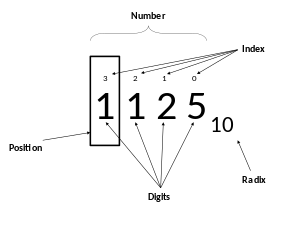
\includegraphics[width=0.5\textwidth]{positional-notation.png}}
    \caption{Glossary of terms used in the positional numeral systems.}
\end{figure}

In any standart positional numeral system, a number is conventionally written as $\left( x \right)_{y} $ with $x$ as the string of digits and $y$ as its base, although for the base 10 the subscript is usually assumed and omitted together with the pair of parenthesis.

Examples of commonly used positional numeral systems include the \textbf{decimal system} (base $10$), the \textbf{binary system} (base $2$) and the \textbf{hexadecimal system} (base $16$).

\begin{definition}
\label{1:pns:num-def}
In a positional numeral system with base $b \left( b > 1 \right) $, a string of digits $d_1\ldots d_n$ denotes the number $d_1b^{n-1} + d_2b^{n-2} + \ldots + d_nb^{0}$, where $0 \le d_i \le b$. 
\end{definition}

In contrast to decimal, or base 10, which as a ones' place, tens' place, hundreds' place, and so on, base $b$ would have a ones' place, then a $b^1$s' place, a $b^2$s' place, etc. 

\begin{proposition}
    A number with $n$ digits with base $b$ can represent $b^n$ different numbers in the range [$0$, $b^n - 1$].
\end{proposition}

\subsubsection{Decimal numeral system}
\begin{definition}
    The decimal numeral system is a positional numeral system with base 10, meaning that it uses 10 digits from 0 to 9.
\end{definition}

In decimal number system, the succesive positions to the left of the decimal point represents units, tens, hundreds, thousands and so on. 

Each position represents a specific power of the base (10). For example, the decimal number 5374 consists of the digit $4$ in the units position, $7$ in the tens position, $3$ in the hundreds position, and $5$ in the thousands position, and by definition \ref{1:pns:num-def} its value can be written as
\begin{equation}
    5\cdot 10^3 + 3\cdot 10^2 + 7\cdot 10^1 + 4\cdot 10^0 = 5000 + 300 + 70 + 4 = 5374
\end{equation}

\begin{proposition}
    A number with $n$ decimal digits from $0$ to $9$ can represent $10^n$ different numbers in the range [$0$, $10^n - 1$].
\end{proposition}

For example, when $n = 3$, $10^3 = 1000$ different numbers can be represented within the range [$0$, $999$].

\subsubsection{Binary numeral system}
\begin{definition}
    The binary numeral system is a positional numeral system with base 2, which uses only two symbols: typically 0 and 1.
\end{definition}

%The binary numeral system (base 2) is used in almost all computers and electronic devices because it's easier to implement efficiently in electronic circuits.

Each binary digit is referred to as a \textbf{bit}. A binary number made up of $4$ binary digits, or $4$ bits, receives the name \textbf{nibble}, and a group of two nibbles, or eight bits, defines what is called a \textbf{byte}.

\begin{proposition}
    A number with $n$ binary digits, $0$ and $1$, can represent $2^n$ different numbers in the range [$0$, $2^n - 1$].
\end{proposition}

For instance, when $n = 3$, $2^3 = 8$ different numbers can be represented within the range [$0$, $7$].

Because of its straightforward implementation in digital electronic circuitry using logic gates, the binary system is used by almost all modern computers and computer-based devices.

%Then, how can we represent analog magnitudes using only 2 possible values?
\newpage
\begin{example}[Convert $10101_2$ from binary to decimal.]
    By definition \ref{1:pns:num-def} we get
    \begin{equation}
        1\cdot 2^4 + 0\cdot 2^3 + 1\cdot 2^2 + 0\cdot 2^1 + 1\cdot 1^0 = 16 + 4 + 1 = 21
    \end{equation}
\end{example}
\begin{example}[Convert $47_{10}$ from decimal to binary.]
    \begin{align}
        47 \quad\%\quad 2 = 1 &\quad\rightarrow\quad 23\quad\%\quad 2 = 1 \quad\rightarrow \\
                              &\quad\rightarrow\quad 11\quad\%\quad 2 = 1 \quad\rightarrow \\
                              &\quad\rightarrow\quad 5\quad\%\quad 2 = 1 \quad\rightarrow \\
                              &\quad\rightarrow\quad 2\quad\%\quad 2 = 0 \quad\rightarrow\quad 2 / 2 = 1
    \end{align}
    Putting the last quotient and the remainders in inverse order we get that $47_{10}$ is $101111_2$ in binary.
\end{example}

\subsubsection{Hexadecimal numeral system}
\begin{definition}
    The hexadecimal system is a positional numeral system with base $16$, commonly used to abbreviate binary numbers.
\end{definition}

The different equivalences in the hexadecimal, decimal and binary systems are shown in the following table.
\bgroup
\def\arraystretch{1.2}
\begin{table}[h!]
\centering
\begin{tabular}{ |c|c|c| }
    \hline
    \textbf{Hexadecimal digit} & \textbf{Decimal equivalent} & \textbf{Binary equivalent} \\
    \hline
    0 & 0 & 0000 \\
    \hline
    1 & 1 & 0001 \\
    \hline
    2 & 2 & 0010 \\
    \hline
    3 & 3 & 0011 \\
    \hline
    4 & 4 & 0100 \\
    \hline
    5 & 5 & 0101 \\
    \hline
    6 & 6 & 0110 \\
    \hline
    7 & 7 & 0111 \\
    \hline
    8 & 8 & 1000 \\
    \hline
    9 & 9 & 1001 \\
    \hline
    A & 10 & 1010 \\
    \hline
    B & 11 & 1011 \\
    \hline
    C & 12 & 1100 \\
    \hline
    D & 13 & 1101 \\
    \hline
    E & 14 & 1110 \\
    \hline
    F & 15 & 1111 \\
    \hline
\end{tabular}
\caption{Hexadecimal, decimal and binary equivalences.}
\label{tbl:hexadecimal-system}
\end{table}
\egroup

\begin{remark}
Note that every hexadecimal digit is a nibble (it's made up of 4 bits).
\end{remark}

\begin{example}[Convert $4AF_{16}$ (or $0x4AF$) from hexadecimal to binary.]
    By looking at table \ref{tbl:hexadecimal-system} we know that
    \begin{equation*}
        4 = 0100 \quad\quad\quad A = 1010 \quad\quad\quad F = 1111
    \end{equation*}
    Then, the hexadecimal number $4AF$ is $010010101111$ in binary.
\end{example}
\begin{example}[Convert $0x4AF$ from hexadecimal to decimal.]
    By definition \ref{1:pns:num-def} between number systems can be do the following operation:
    \begin{align*}
        4AF &= 4\cdot 16^2  + 10\cdot 16^1 + 15\cdot 16^0 =  4\cdot 2^8 + 160 + 15 \\
            &= 4\cdot 256 + 160 + 15 = 1199
    \end{align*}
\end{example}

\subsection{Axioms, theorems and properties of Boolean algebra}

%\subsubsection{Basic boolean algebra properties and laws}
Boolean algebra is a mathematical tool used for analysis and synthesis of binary digital systems. It's named after George Bool, a british mathematician from the $19^{th}$ century.

\begin{definition}
    A boolean variable is a digital signal which only has 1 out of 2 possible values in an instant, which are mutually exclusive. Those values are usually represented as 0 and 1, but another representation could be OFF and ON, or HIGH and LOW.
\end{definition}
\begin{definition}
    Let $A$ be a Boolean variable. We call $A$ the \textbf{true form} of the variable and $\overline{A}$, its inverse, the \textbf{complementary form}. $\overline{A}$ is the complement of $A$.
\end{definition}
\begin{note}
    The "true form" of a variable does not mean that $A$ is true, but merely that $A$ does not have a line over it.
\end{note}

\bgroup
\def\arraystretch{1.5}
\def\tabcolstep{20}
\begin{table}[h!]
\centering
\begin{tabular}{ |c|c|c| }
    \hline 
    \textbf{Name} & \textbf{Property} & \textbf{Dual} \\
    \hline
    Indentity & $B\cdot 1 = B$ & $B + 0 = B$ \\
    \hline
    Annulment & $B\cdot 0 = 0$ & $B + 1 = 1$ \\
    \hline
    Idempotent & $B\cdot B = B$ & $B + B = B$ \\
    \hline
    Double negation & $\overline{\overline{B}} = B$ & $\overline{\overline{B}}$ \\
    \hline
    Complement & $B\cdot\overline{B}$ = 0 & $B + \overline{B} = 1$ \\
    \hline
    Commutative & $B\cdot C = C\cdot B$ & $B + C = C + B$ \\ 
    \hline
    Associative & $\left( B\cdot C \right)\cdot D = B\cdot\left( C\cdot D \right)$ & $\left( B + C \right) + D = B + \left( C + D \right)$ \\
    \hline
    Distributive & $\left( B\cdot C \right) + \left( B\cdot D \right) = B\cdot\left( C + D \right)$ & $\left( B + C \right)\cdot\left( B + D \right) = B + \left( C\cdot D \right)$ \\
    \hline
\end{tabular}
\caption{Basic properties of boolean algebra.}
\end{table}
\egroup

\begin{definition}
    \textbf{(De Morgan's laws).} De Morgan's laws let us the operations in the expression we are working with.
\begin{equation}
    \left(\overline{B_0\cdot B_1\cdot\ldots\cdot B_{n-1}} \right) = \left( \overline{B_0} + \overline{B_1} + \ldots + \overline{B_{n-1}} \right)
\end{equation} 
\begin{equation}
    \left( \overline{B_0 + B_1 + \ldots + B_{n-1}} \right) = \left( \overline{B_0}\cdot\overline{B_1}\cdot\ldots\cdot\overline{B_{n-1}} \right)  
\end{equation}
\end{definition}


\subsection{Basic Boolean algebraic operations and logic gates}
\begin{definition}
    Let $A$ and $B$ be two Boolean variables
\end{definition}

%\subsection{Boolean expressions and operations. Logic functions and gates}
\begin{definition}
    A logic function is a circuit accepting at least one input logical value and outputs a logical value.
\end{definition}

In order to describe the working principle of a logic function a \textbf{truth table} is used. In this table is specified all the posible outputs for all possible input logic values. Also it's a graphical representation of all cases that can happen in an algebraic relation and its respective results.
\begin{table}[h!]
\centering
\begin{tabular}{ |c|c|c| }
    \hline 
    \textbf{A} & \textbf{B} & \textbf{Output} \\
    \hline
    0 & 0 & 0 \\
    0 & 1 & 1 \\
    1 & 0 & 1 \\
    1 & 1 & 0 \\
    \hline
\end{tabular}
\caption{Example of a truth table. In this case is a XOR logic gate.}
\end{table}

\begin{definition}
    Logic gates are the implementation of most basic logic functions.
\end{definition}

\paragraph{Amplifier / BUFFER gate}
\begin{definition} The amplifier, or most commonly named, the BUFFER, is the simplest logic gate. It expects one input (A) and gives one output value (Z).
\end{definition}

It follows the logic equation $Z = A$, meaning the input received by the buffer is not changed at all, and its corresponding truth table is the following one.

\begin{minipage}{\textwidth}
\vspace{1cm}
\begin{minipage}[c]{0.49\textwidth}
    \centering
    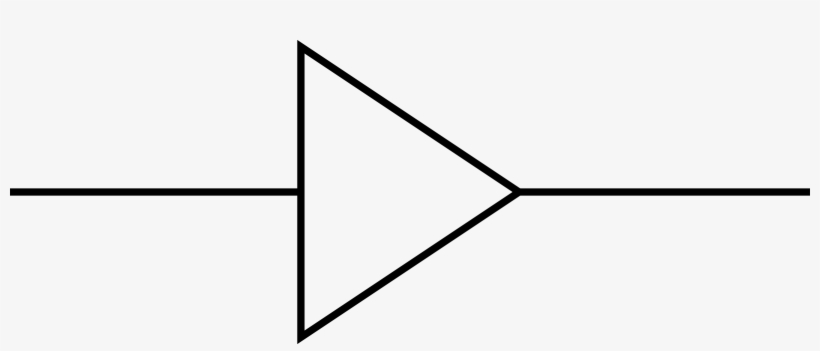
\includegraphics[width=.5\textwidth]{buffer-gate.png}
    \captionof{figure}{Graphical representation of a BUFFER.}
\end{minipage}
\hfill
\begin{minipage}[c]{.49\textwidth}
    \centering
    \begin{tabular}{ |c|c| } \hline 
        \textbf{A} & \textbf{Z} \\ \hline
        1 & 1 \\
        0 & 0 \\
        \hline
    \end{tabular}
    \captionof{table}{Truth table for a BUFFER.}
\end{minipage}
\end{minipage}

\hide{
\begin{table}[h!]
\centering
\begin{tabular}{ |c|c| }
    \hline 
    \textbf{A} & \textbf{Z} \\
    \hline
    1 & 1 \\
    0 & 0  \\
    \hline
\end{tabular}
\caption{Truth table for a BUFFER gate.}
\end{table}

\begin{figure}[htbp]
    \centerline{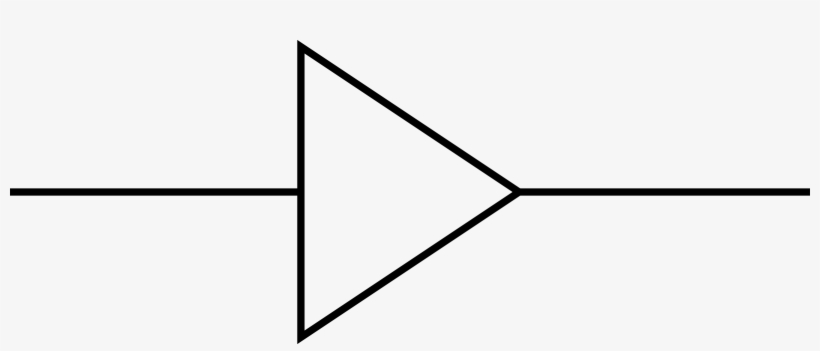
\includegraphics[width=0.35\textwidth]{buffer-gate.png}}
    \caption{Graphical representation of a BUFFER gate.}
\end{figure}
}

\newpage
\paragraph{NOT gate / Inverter}
\begin{definition} The NOT gate, also called an \textbf{inverter}, gets one input value (A) and gives the opposite output value (Z), following the logic equation $Z = \overline{A}$.
\end{definition}

\begin{minipage}{\textwidth}
\vspace{1cm}
\begin{minipage}[c]{0.49\textwidth}
    \centering
    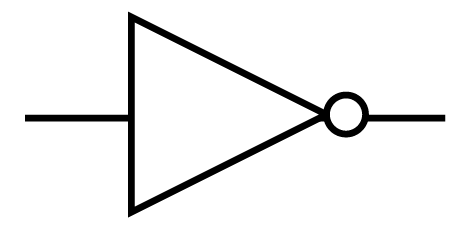
\includegraphics[width=.5\textwidth]{not-gate.png}
    \captionof{figure}{Graphical representation of a NOT gate.}
\end{minipage}
\hfill
\begin{minipage}[c]{.49\textwidth}
    \centering
    \begin{tabular}{ |c|c| } \hline 
        \textbf{A} & \textbf{Z} \\ \hline
        1 & 0 \\
        0 & 1 \\
        \hline
    \end{tabular}
    \captionof{table}{Truth table for a NOT gate.}
\end{minipage}
\end{minipage}

\hide{
\begin{figure}[htbp]
    \centerline{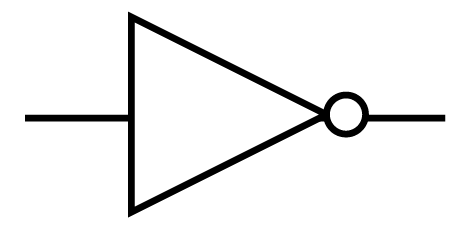
\includegraphics[width=0.3\textwidth]{not-gate.png}}
    \caption{Graphical representation of a NOT logic gate.}
\end{figure}
\begin{table}[h!]
\centering
\begin{tabular}{ |c|c| } \hline 
    \textbf{A} & \textbf{Z} \\
    \hline
    1 & 0 \\
    0 & 1 \\
    \hline
\end{tabular}
\caption{Truth table for a NOT gate.}
\end{table}
}

\paragraph{AND gate / Boolean multiplication}
%\begin{minipage}[c]{.45\textwidth}
\begin{definition} 
    \textbf{(AND gate / Logical AND).} The AND gate gets at least two input values (A, B) and gives the one output value (Z). The output value Z will be true, $Z = 1$, if and only if both inputs $A$ and $B$ are simultaneously true. 
\end{definition}
%\newpage
The logic equation corresponding to the AND gate is $Z = A\cdot B$. Looking at this equation we could see the AND gate as a multiplication operation.

\begin{minipage}{\textwidth}
\vspace{1cm}
\begin{minipage}[c]{0.49\textwidth}
    \centering
    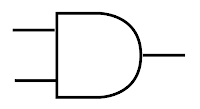
\includegraphics[width=.5\textwidth]{and-gate.png}
    \captionof{figure}{Graphical representation of an AND gate.}
\end{minipage}
\hfill
\begin{minipage}[c]{.49\textwidth}
    \centering
    \begin{tabular}{ |c|c|c| } \hline 
        \textbf{A} & \textbf{B} & \textbf{Z} \\ \hline
        0 & 0 & 0 \\
        0 & 1 & 0 \\
        1 & 0 & 0 \\
        1 & 1 & 1 \\ 
        \hline
    \end{tabular}
    \captionof{table}{Truth table for an AND gate.}
\end{minipage}
\end{minipage}

%\blindtext
\hide{
\begin{figure}[htbp]
\begin{floatrow}
\ffigbox{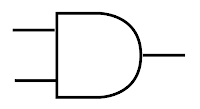
\includegraphics[width=.3\textwidth]{and-gate.png}}{\caption{Graphical representation of an AND gate.}}
\capbtabbox{%
\begin{tabular}{ |c|c|c| }
    \hline 
    \textbf{A} & \textbf{B} & \textbf{Z} \\
    \hline
    0 & 0 & 0 \\
    0 & 1 & 0 \\
    1 & 0 & 0 \\
    1 & 1 & 1 \\
    \hline
\end{tabular}
}{\caption{Truth table for an AND gate.}}
\end{floatrow}
\end{figure}
}
%\hide{
%\begin{figure}[htbp]
%\end{minipage}
%\begin{minipage}[c]{.45\textwidth}
%\begin{subfigure}{.5\textwidth}
%\begin{table}[h!]
%\centering
%\begin{tabular}{ |c|c|c| }
%    \hline 
%    \textbf{A} & \textbf{B} & \textbf{Z} \\
%    \hline
 %   0 & 0 & 0 \\
%    0 & 1 & 0 \\
%    1 & 0 & 0 \\
%    1 & 1 & 1 \\
%    \hline
%\end{tabular}
%\caption{Truth table for an AND gate.}
%\end{table}
%\end{subfigure}
%\begin{figure}[htbp]
%    \begin{subfigure}{.5\textwidth}
%    \centerline{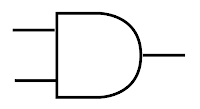
\includegraphics[width=\textwidth]{and-gate.png}}
%    \caption{Graphical representation of an AND logic gate.}
%\end{figure}
%\end{figure}
%\end{minipage}
%}

\paragraph{OR gate / Boolean addition}
\begin{definition} The OR gate gets a minimum of two input values (A, B) and gives the one output value (Z). The output value Z will be true, $Z = 1$, if at least one of the inputs $A$ and $B$ is true. 
\end{definition}

Then, the logic equation corresponding to the OR gate is $Z = A + B$. Looking at this equation we could see the OR gate as an addition operation.

\begin{minipage}{\textwidth}
\vspace{1cm}
\begin{minipage}[c]{0.49\textwidth}
    \centering
    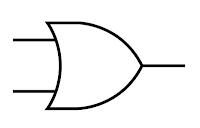
\includegraphics[width=.5\textwidth]{or-gate.png}
    \captionof{figure}{Graphical representation of an OR gate.}
\end{minipage}
\hfill
\begin{minipage}[c]{.49\textwidth}
    \centering
    \begin{tabular}{ |c|c|c| } \hline 
        \textbf{A} & \textbf{B} & \textbf{Z} \\ \hline
        0 & 0 & 0 \\
        0 & 1 & 1 \\
        1 & 0 & 1 \\
        1 & 1 & 1 \\
        \hline
    \end{tabular}
    \captionof{table}{Truth table for an OR gate.}
\end{minipage}
\end{minipage}

\hide{
\begin{figure}[htbp]
    \centerline{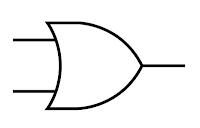
\includegraphics[width=0.3\textwidth]{or-gate.png}}
    \caption{Graphical representation of an OR logic gate.}
\end{figure}
\begin{table}[h!]
\centering
\begin{tabular}{ |c|c|c| }
    \hline 
    \textbf{A} & \textbf{B} & \textbf{Z} \\
    \hline
    0 & 0 & 0 \\
    0 & 1 & 1 \\
    1 & 0 & 1 \\
    1 & 1 & 1 \\
    \hline
\end{tabular}
\caption{Truth table for an OR gate.}
\end{table}
}


\paragraph{NAND gate / Inverted AND gate}
\begin{definition}
    A NAND gate is a type of logic gate that gets at least two input values (A, B) and gives one output value (Z), which is 1 if at least one of the inputs is 0.
\end{definition}

This logic gate can be though as a combination of an AND and a NOT gates, i.e. an inverted AND gate, and its corresponding logic equation is $Z = \overline{A\cdot B}$.
\begin{note}
    $Z = \overline{A\cdot B}$ is not the same as $Z = \overline{A}\cdot\overline{B}$.
\end{note}

\begin{minipage}{\textwidth}
\vspace{1cm}
\begin{minipage}[c]{0.49\textwidth}
    \centering
    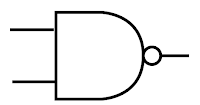
\includegraphics[width=.5\textwidth]{nand-gate.png}
    \captionof{figure}{Graphical representation of a NAND gate.}
\end{minipage}
\hfill
\begin{minipage}[c]{.49\textwidth}
    \centering
    \begin{tabular}{ |c|c|c| } \hline 
        \textbf{A} & \textbf{B} & \textbf{Z} \\ \hline
        0 & 0 & 1 \\
        0 & 1 & 1 \\
        1 & 0 & 1 \\
        1 & 1 & 0 \\
        \hline
    \end{tabular}
    \captionof{table}{Truth table for a NAND gate.}
\end{minipage}
\end{minipage}

\hide{
\begin{figure}[htbp]
    \centerline{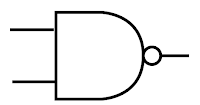
\includegraphics[width=0.25\textwidth]{nand-gate.png}}
    \caption{Graphical representation of a NAND logic gate.}
\end{figure}
\begin{table}[h!]
\centering
\begin{tabular}{ |c|c|c| }
    \hline 
    \textbf{A} & \textbf{B} & \textbf{Z} \\
    \hline
    0 & 0 & 1 \\
    0 & 1 & 1 \\
    1 & 0 & 1 \\
    1 & 1 & 0 \\
    \hline
\end{tabular}
\caption{Truth table for a NAND gate.}
\end{table}
}

\paragraph{NOR gate / Inverted OR gate}
\begin{definition}
    A NOR gate is a type of logic gate that gets at least two input values (A, B) and gives one output value (Z), which is 1 if both inputs are 0, and is 0 if at least one of the inputs is 1.
\end{definition}

The corresponding logic equation for a NOR gate is $Z = \overline{A + B}$.

\begin{minipage}{\textwidth}
\vspace{1cm}
\begin{minipage}[c]{0.49\textwidth}
    \centering
    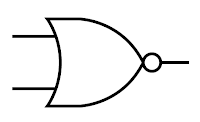
\includegraphics[width=.5\textwidth]{nor-gate.png}
    \captionof{figure}{Graphical representation of a NOR gate.}
\end{minipage}
\hfill
\begin{minipage}[c]{.49\textwidth}
    \centering
    \begin{tabular}{ |c|c|c| } \hline 
        \textbf{A} & \textbf{B} & \textbf{Z} \\ \hline
        0 & 0 & 1 \\
        0 & 1 & 0 \\
        1 & 0 & 0 \\
        1 & 1 & 0 \\        
        \hline
    \end{tabular}
    \captionof{table}{Truth table for a NOR gate.}
\end{minipage}
\end{minipage}

\hide{
\begin{figure}[htbp]
    \centerline{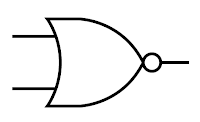
\includegraphics[width=0.25\textwidth]{nor-gate.png}}
    \caption{Graphical representation of a NOR logic gate.}
\end{figure}

\begin{table}[h!]
\centering
\begin{tabular}{ |c|c|c| }
    \hline 
    \textbf{A} & \textbf{B} & \textbf{Z} \\
    \hline
    0 & 0 & 1 \\
    0 & 1 & 0 \\
    1 & 0 & 0 \\
    1 & 1 & 0 \\
    \hline
\end{tabular}
\caption{Truth table for a NOR gate.}
\end{table}
}

\paragraph{XOR gate / OR-exclusive gate}
\begin{definition}
    A XOR gate, or OR-exclusive gate, is a type of logic gate that gets at least two input values (A, B) and gives one output value (Z), which is 1 if and only if one input is 1.
\end{definition}

The XOR gate can be seen as a comparator of bits (if both bits are equal the output is 0); and its corresponding logic equation is $Z = A\oplus B$.

\begin{minipage}{\textwidth}
\vspace{1cm}
\begin{minipage}[c]{0.49\textwidth}
    \centering
    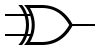
\includegraphics[width=.5\textwidth]{xor-gate.png}
    \captionof{figure}{Graphical representation of a XOR gate.}
\end{minipage}
\hfill
\begin{minipage}[c]{.49\textwidth}
    \centering
    \begin{tabular}{ |c|c|c| } \hline 
        \textbf{A} & \textbf{B} & \textbf{Z} \\ \hline
        0 & 0 & 0 \\
        0 & 1 & 1 \\
        1 & 0 & 1 \\
        1 & 1 & 0 \\       
        \hline
    \end{tabular}
    \captionof{table}{Truth table for a XOR gate.}
\end{minipage}
\end{minipage}

\hide{
\begin{figure}[htbp]
    \centerline{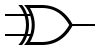
\includegraphics[width=0.25\textwidth]{xor-gate.png}}
    \caption{Graphical representation of a XOR logic gate.}
\end{figure}
\begin{table}[h!]
\centering
\begin{tabular}{ |c|c|c| }
    \hline 
    \textbf{A} & \textbf{B} & \textbf{Z} \\
    \hline
    0 & 0 & 0 \\
    0 & 1 & 1 \\
    1 & 0 & 1 \\
    1 & 1 & 0 \\
    \hline
\end{tabular}
\caption{Truth table for a XOR gate.}
\end{table}
}

\paragraph{XNOR gate / Inverted OR-exclusive gate}
\begin{definition}
    A XNOR gate is a type of logic gate that gets two input values (A, B) and gives one output (Z), which is 0 if and only if one input is 0.
\end{definition}

The corresponding logic equation for a XNOR gate is $Z = \overline{A\oplus B}$.

\begin{minipage}{\textwidth}
\vspace{1cm}
\begin{minipage}[c]{0.49\textwidth}
    \centering
    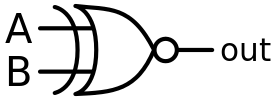
\includegraphics[width=.5\textwidth]{xnor-gate.png}
    \captionof{figure}{Graphical representation of a XNOR gate.}
\end{minipage}
\hfill
\begin{minipage}[c]{.49\textwidth}
    \centering
    \begin{tabular}{ |c|c|c| } \hline 
        \textbf{A} & \textbf{B} & \textbf{Z} \\ \hline
        0 & 0 & 1 \\
        0 & 1 & 0 \\
        1 & 0 & 0 \\
        1 & 1 & 1 \\ 
        \hline
    \end{tabular}
    \captionof{table}{Truth table for a XNOR gate.}
\end{minipage}
\end{minipage}

\hide{
\begin{figure}[htbp]
    \centerline{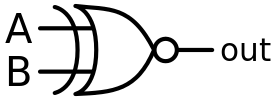
\includegraphics[width=0.25\textwidth]{xnor-gate.png}}
    \caption{Graphical representation of a XNOR logic gate.}
\end{figure}
\begin{table}[h!]
\centering
\begin{tabular}{ |c|c|c| }
    \hline 
    \textbf{A} & \textbf{B} & \textbf{Z} \\
    \hline
    0 & 0 & 1 \\
    0 & 1 & 0 \\
    1 & 0 & 0 \\
    1 & 1 & 1 \\
    \hline
\end{tabular}
\caption{Truth table for a XNOR gate.}
\end{table}
}

\subsection{Logic circuits and Boolean functions}
\begin{definition}
    \textbf{(Logic circuit).} A logic circuit is the combination of different logic gates by taking the output from one gate and using it as the input to another gate. It is composed of inputs, outputs, its functional specification and its temporal specification (delay)
\end{definition}

\begin{figure}[htbp]
    \centerline{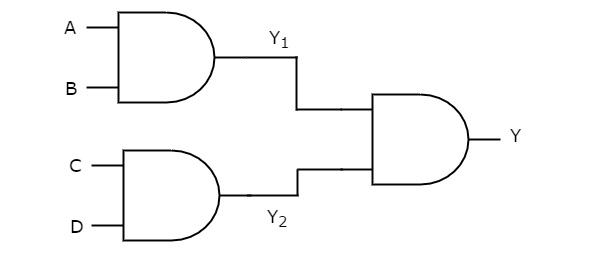
\includegraphics[width=0.5\textwidth]{logic-circuit.jpg}}
    \caption{Example of a logic circuit that takes four inputs (A, B, C, D) and gives one output (Y). In this case, the functional specification for this logic circuit is 
    %\begin{equation}
    $Y_1 = \left( A, B \right)\quad\quad Y_2 = \left( C, D \right) \quad\quad Y\left( Y_1, Y_2 \right)$}
    %\end{equation}}
    %\label{1:lc:ex}
\end{figure}

%Digital circuits are classified as \textbf{combinational} or \textbf{sequential}. 

Logic circuits enables computers to do more complex operations than they could accomplish with just a single gate. 

\begin{definition}
    \textbf{(Combinational circuit).} A combinational circuit is the one whose outputs depend only on the current values of the inputs; i.e. it combines the current input values to compute the output. For example, a logic gate is a combinational circuit. 
\end{definition}
\begin{definition}
    \textbf{(Sequential circuit).} A sequential circuit is the one whose outputs depend on both current and previous values of the inputs; i.e. it depends on the input sequence. A combinational circuit is memoryless, but a sequential one has memory.
\end{definition}

The functional specification of a logic circuit is usually expressed as a truth table or a Boolean function. 

%In the next sections is described how to derive a Boolean function from any truth table and how to use Boolean Algebra and Karnaugh maps to simplify those functions.

\begin{definition}
    \textbf{(Boolean function).} A Boolean function is an expression that relates Boolean variables, in other words, it takes at least one variable (or literal) and gives and output value that can be either TRUE or FALSE.
\end{definition}

\begin{definition}
    \textbf{(Implicant).} The AND of one or more literals is called a \textbf{product} or an \textbf{implicant}.
\end{definition}
\begin{definition}
    \textbf{(Minterm).} A minterm is a product involving all of the inputs to the function. 
\end{definition}

For instance, $A\overline{B}C$ is a minterm for a function of the three variables $A$, $B$ and $C$, but $\overline{A}B$ is not, because it doesn't involve $C$.

\begin{definition}
    \textbf{(Sum).} Similarly, the OR of one or more literals is called a \textbf{sum}.
\end{definition}
\begin{definition}
    \textbf{(Maxterm).} A maxterm is a sum involving all of the inputs to the function. 
\end{definition}

For example, $A + \overline{B} + C$ is a maxterm for a function of the three variables $A$, $B$ and $C$.

\begin{note}
    Minterms and maxterms are dual concepts because of their complementary-symmetry relationship as expressed by De Morgan's laws.
\end{note}

\subsubsection{Canonical disjunctive normal form (SOP form)}
A truth table of $n$ inputs contains $2^n$ rows, one for each possible value of the inputs. Each row in a truth table is associated with a minterm that is TRUE for that row, and only for that row. We can write a Boolean function for any truth table by summing each of the minterms for which the output is TRUE.

In table \ref{1:lf:sop-tt}, for instance, the minterm for the first row is $\overline{A}\ \overline{B}$ because that expression is TRUE when $A = 0$ and $B = 0$. 
\bgroup
\def\arraystretch{1.3}
\begin{table}[h!]
\centering
\begin{tabular}{|c|c|c|c|c|}
    \hline
    \textbf{A} & \textbf{B} & \textbf{Y} & \textbf{Minterm} & \textbf{Index} \\
    \hline
    0 & 0 & 0 & $\overline{A}\ \overline{B}$ & 0 \\
    0 & 1 & 1 & $\overline{A}B$ & 1 \\
    1 & 0 & 0 & $A\overline{B}$ & 2\\
    1 & 1 & 1 & $AB$ & 3 \\
    \hline
\end{tabular}
\caption{Truth table with multiple TRUE minterms.}
\label{1:lf:sop-tt}
\end{table}
\egroup

For the truth table \ref{1:lf:sop-tt}, taking the sum of each of the minterms (or rows) for which the output $Y$ is TRUE gives $Y = \overline{A}B + AB$. This is called the \textbf{canonical disjunctive normal form}, or \textbf{sum-of-products (SOP) canonical form} of a function because it is the sum (OR) of products (ANDs forming minterms), and can be expressed as
\begin{equation}
    Y = F\left( A, B \right) = \sum m_i,\ i\in \{1, 3\} = \overline{A}B + AB 
\end{equation}
where $m_i$ are the minterms to map.

\begin{note}
    \textit{Canonical form} is just a fancy word for standard form.
\end{note}
\begin{note}
The term SOP (Sum of Products) is widely used for the canonical form that its a disjunction (OR) of minterms.
\end{note}

The SOP form provides a Boolean function for any truth table with any number of variables. Unfortunately, SOP form doesn't necessarily generate the simplest function. We can use Boolean algebra properties and laws to simplify the expression or use Karnaugh maps to get the simplest one directly from the truth table.

\subsubsection{Canonical conjunctive normal form (POS form)}
An alternative way of expressing Boolean functions is the \textbf{canonical conjunctive normal form}, or \textbf{product-of-sums (POS) canonical form}. Each row of a truth table corresponds to a maxterm that is FALSE for that row. For example, the maxterm for the first row of a two-input truth table is $\left( A + B \right)$ because $\left( A + B \right)$ is FALSE when $A = 0$ and $B = 0$, and its expressed as
\begin{equation}
    Y = F\left( A, B \right) = \prod M_i,\ i\in \{0\} = A + B 
\end{equation}
where $M_i$ are the maxterms to map.

SOP produces the shortest functions when the output is TRUE on only a few rows of a truth table; POS is simpler when the output is FALSE on only a few rows of a truth table.






%%%%%%%%%%%%%%%%%%%%%%%%%%%%%%
%%%%% SHEEEEEEEEEEEEEEEEET %%%%%%%%%%%%%
%%%%%%%%%%%%%%%%%%%%%%%%%%%%%%
\hide{
\newpage
\subsection{Logic circuits and implementation of logic functions}
%Computers often chain logic gates together by taking the output from one gate and using it as the input to another gate. We call that a \textbf{logic circuit}. Circuits enables computers to do more complex operations than they could accomplish with just a single gate.
\begin{definition}
    The combination of different logic gates by taking the output from one gate and using it as the input to another gate is called a \textbf{logic circuit}. 
\end{definition}

A logic circuit is composed of inputs, outputs, its functional specification and its temporal specification (delay).

Logic circuits enables computers to do more complex operations than they could accomplish with just a single gate. 

\begin{note}
    Any logic function can be expressed using AND, OR and NOT gates.
\end{note}
\begin{figure}[htbp]
    \centerline{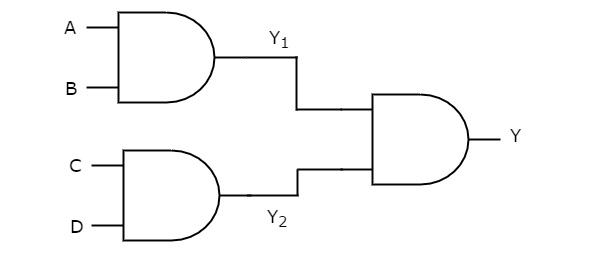
\includegraphics[width=0.5\textwidth]{logic-circuit.jpg}}
    \caption{Example of a logic circuit that takes four inputs (A, B, C, D) and gives one output (Y). In this case, the functional specification for this logic circuit is \begin{equation}
    Y_1 = \left( A, B \right)\quad\quad Y_2 = \left( C, D \right) \quad\quad Y\left( Y_1, Y_2 \right)   
\end{equation}
    }
    \label{1:lc:ex}
\end{figure}

\begin{definition}
    Combinational logic circuits are the ones in which the output state depends exclusively on input states, i.e. it's a circuit without memory.
\end{definition}
\begin{definition}
    Sequential logic circuits are the ones in which the output state also depends on the previous state of the system, i.e. it's a circuit with memory.
\end{definition}

In Boolean algebra, any Boolean function can be put into the \textbf{canonical disjunctive normal form} (CDNF) or \textbf{minterm canonical form} and into its dual \textbf{canonical conjunctive normal form} (CCNF) or \textbf{maxterm canonical form}.

Minterms are called products because they are the logical AND of a set of variables, and maxterms are called sums because they are the logical OR of a set of variables. These concepts are dual because of their complementary-symmetry relationship as expressed by De Morgan's laws.

Two dual canonical form of any Boolean function are a \textbf{sum of minterms} and a \textbf{product of maxterms}. The term SOP is widely used for the canonical form that its a disjunction (OR) of minterms. Its De Morgan dual is a \textbf{Product of Sums (POS)} for the canonical form that is a conjunction (AND) of maxterms, These forms can be useful for the simplification of these functionss, which is of great importance in the optimization of Boolean formulas in general and digital circuits in particular.


\subsubsection{Canonical form of a logic function}
\begin{definition}
    A logic function is a boolean expression that relates logic variables by the use of AND and OR operations, or logic gates.
\end{definition}

In boolean algebra, a boolean function can be expressed as a \textbf{canonical disjunctive normal form} known as \textbf{minterm} or in \textbf{canonical conjunctive normal form} known as \textbf{maxterm}.

Logic functions are represented as logic circuits with 2 levels whose \textbf{canonical form} can be
\begin{itemize}
    \item Sum of Products of all variables or their conjugates: Sum of Minterms or SOP circuits (Sum of Products).
    \item Product of Sums of all variables or their conjugates: Product of Maxterms or POS circuits (Products of Sums).
\end{itemize}
\begin{note}
    All boolean equations can be represented as a sum of minterms (SOP).
\end{note}
\begin{definition}
    Each row of a truth table is a minterm. A minterm is a product (AND) of variables and their complement. Each minterm is true for that row, and only for that row.
\end{definition}

Function is constructed as the sum (OR) of minterms whose output is true. It's then a sum of products.

\bgroup
\def\arraystretch{1.3}
\def\tabcolstep{30}
\begin{table}[h!]
\centering
\begin{tabular}{ |c|c|c|c|c| }
    \hline 
    \textbf{A} & \textbf{B} & \textbf{Y} & \textbf{Minterm} & \textbf{Index} \\
    \hline
    0 & 0 & 0 & $\overline{A}\cdot\overline{B}$ & 0 \\
    0 & 1 & 1 & $\overline{A}\cdot B$ & 1 \\
    1 & 0 & 0 & $A\cdot\overline{B}$ & 2 \\
    1 & 1 & 1 & $A\cdot B$ & 3 \\
    \hline
\end{tabular}
\caption{$Y = F\left( A, B \right) = \overline{A}B + AB$.}
\end{table}
\egroup

\begin{definition}
    \textbf{(Standard form of a logic function).} A boolean variable can be expressed in either true form or complemented form. In standard form a boolean function will contain all the variables in either true form or complemented form while in canonical the number of variables depends on the output of the SOP or POS.
\end{definition}



\subsubsection{Extension to multiple entries}

\subsubsection{Functional habilitation}

\subsubsection{SOP and POS gates implementation}

}
%%%%%%%%%%%%%END SHEEET %%%%%%%%%%%%55
%%%%%%%%%%%%%%%%%%%%%%%%%%%%%5
%%%%%%%%%%%%%%%%%%%%%%%%%%%%%


\subsection{Karnaugh diagrams}
\begin{definition}
    \textbf{(Karnaugh maps).} Karnaugh maps (K-maps) are a graphical method for simplifying Boolean functions consisting on a sequence of cells where each one represents the binary value of an input. These cells are arranged so that the simplification of an expression consists on grouping adecuately the cells.
\end{definition}
\begin{proposition}
    For an expression of $n$ variables $2^n$ cells are needed in the corresponding Karnaugh map.
\end{proposition}

Karnaugh maps make easier the planning of logic designs with simpler gate structure, leading to a more economic design; and can be used for expressions of up to 6 variables. For higher number of variables other methods such as the Quine-McClusky or CAD methods are used.

\begin{definition}
    \textbf{(Adjacent cells).} Cells in a K-map whose values differ only in one variable. Adjacent cells have a Hamming distance of 1.
\end{definition}

Cells on a K-map are disposed so that only one variable changes in between adjacent cells. Physically, each cell is adjacent to every inmediate next cell (4 sides). 

\begin{note}
    Cells cannot be adjacent diagonally.
\end{note}

\begin{definition}
    \textbf{(Cyclical adjacency).} Upper cells are adjacent to its inmmediate lower cells and left cells are adjacent to its inmediate right.
\end{definition}

Given the truth table for a function $Y = F\left( A, B, C \right) $ of variables $A$, $B$ and $C$, the corresponding K-map is a matrix of 8 cells in which binary values of $A$ and $B$ are located on the left and $C$ ones on the top.

\begin{minipage}{\textwidth}
\vspace{1cm}
\begin{minipage}[c]{0.49\textwidth}
    \centering
    \def\arraystretch{1.2}
    \begin{tabular}{ |c|c|c|c| } \hline 
        \textbf{A} & \textbf{B} & \textbf{C} & \textbf{Y} \\ \hline
        0 & 0 & 0 & 1 \\
        0 & 0 & 1 & 1 \\
        0 & 1 & 0 & 0 \\
        0 & 1 & 1 & 0 \\
        \hline
        1 & 0 & 0 & 1 \\
        1 & 0 & 1 & 0 \\
        1 & 1 & 0 & 1 \\
        1 & 1 & 1 & 0 \\
        \hline
    \end{tabular}
    $\quad\quad\longrightarrow$
\end{minipage}
\hfill
\begin{minipage}[c]{.49\textwidth}
    \centering
    \begin{karnaugh-map}[2][4][1][$C$][$AB$]
    \manualterms{1, 1, 0, 0, 1, 0, 1, 0}
    \minterms{1, 2}
    %\implicant{0}{1}
    %\implicant{6}{4}
\end{karnaugh-map}
\end{minipage}
\end{minipage}

For instance, when $A = 0$, $B = 0$ and $C = 0$ the function has value 1, which corresponds in this case to the minterm $\overline{A}\cdot\overline{B}\cdot\overline{C}$.

\subsubsection{SOP minimization through K-map}
For every term of the SOP expression a 1 is added in the K-map cell correspondent to the product value. Then, taking the previous truth table,

\begin{minipage}{\textwidth}
\vspace{1cm}
\begin{minipage}[c]{0.49\textwidth}
    \centering
    \def\arraystretch{1.2}
    \begin{tabular}{ |c|c|c|c|c|c| } \hline 
        \textbf{A} & \textbf{B} & \textbf{C} & \textbf{Y} & \textbf{Minterm} & \textbf{Index} \\ \hline
        0 & 0 & 0 & 1 & $\overline{A}\cdot\overline{B}\cdot\overline{C}$ & 0 \\
        0 & 0 & 1 & 1 & $\overline{A}\cdot\overline{B}\cdot C$ & 1 \\
        0 & 1 & 0 & 0 & $\overline{A}\cdot B\cdot\overline{C}$ & 2 \\
        0 & 1 & 1 & 0 & $\overline{A}\cdot B\cdot C$ & 3 \\
        \hline
        1 & 0 & 0 & 1 & $A\cdot\overline{B}\cdot\overline{C}$ & 4 \\
        1 & 0 & 1 & 0 & $A\cdot\overline{B}\cdot C$ & 5 \\
        1 & 1 & 0 & 1 & $A\cdot B\cdot\overline{C}$ & 6 \\
        1 & 1 & 1 & 0 & $A\cdot B\cdot C$ & 7 \\
        \hline
    \end{tabular}
    $\quad\longrightarrow$
\end{minipage}
\hfill
\begin{minipage}[c]{.49\textwidth}
    \centering
    \begin{karnaugh-map}[2][4][1][$C$][$AB$]
    \manualterms{1, 1, 0, 0, 1, 0, 1, 0}
    \minterms{1, 2}
    \implicant{0}{1}
    \implicant{6}{4}
    \end{karnaugh-map}
\end{minipage}
\end{minipage}

the SOP expression for the function described by the truth table is 
\begin{equation}
    Y = \sum m_i,\ i\in \{0, 1, 5, 7\} = \overline{A}\cdot\overline{B}\cdot\overline{C} + \overline{A}\cdot\overline{B}\cdot C + A\cdot\overline{B}\cdot C + A\cdot B\cdot C
\end{equation}

As one may see, this expression taken directly from the truth table is not simplified at all. In order to simplify the SOP expression after obtaining the K-map 3 steps should be followed:
\begin{enumerate}
    \item \textbf{One's grouping.} A group has to contain 1, 2, 4, 8 or 16 cells, i.e. a power of 2 cells. For example, a K-map of 3 variables would have a maximum group of 8 cells.

        Each cell of a group has to be adjacent to one or more cells of the same group, but not all cells of the group must be adjacent to each other.

        We should maximize the number of 1s in each group.

        Each 1 of the map has to be included in, at least, one group. 1s already in a group can be included into other groups given that the overlaping groups contains non common 1s.
        \begin{center}
        \begin{karnaugh-map}[4][4][1][$CD$][$AB$]
            \manualterms{1, 0, 1, 0, 1, 1, 1, 0, 1, 0, 1, 1, 1, 1, 1, 0}
            %\minterms{3, 4}
            \implicant{4}{13}
            \implicant{11}{10}
            %\implicantcorner
            \implicantedge{0}{8}{2}{10}
            %\implicant{11}{10}
        \end{karnaugh-map}
        \end{center}

    \item\textbf{Determination of each term of the SOP.} Each group of cells containing 1s gives one product term composed of all variables appearing in the group in only one form (complemented or non complemented).

        Variables complemented and non complemented inside the same group are deleted.

    \item\textbf{SOP terms obtained.} Once obtained all minimum terms form the K-map they are added up to obtaine the minimal product expression.
\end{enumerate}

\begin{note}
    In case we have a non-standard SOP with a term that lacks one or more variables to its expression it must be completed by counting all the possible terms.
\end{note}


\subsubsection{POS minimization through K-map}
The minimization process of a POS is basically the same as that for SOP although now the 0s are to be grouped to create the minimum number of sum terms. Rules applied to group 0s are the same as those to group 1s.
